\documentclass[11pt,a4paper]{article}
\usepackage[T1]{fontenc}
\usepackage[utf8]{inputenc}
\usepackage{lmodern}
\usepackage{amsmath,amssymb,amsthm,mathtools,mathrsfs}
\usepackage{graphicx,float,xcolor,multicol}
\usepackage[shortlabels]{enumitem}
\usepackage[margin=27mm]{geometry}
\usepackage{microtype,needspace,placeins}
\usepackage{tikz,tikz-cd}
\usetikzlibrary{arrows.meta,calc,positioning,patterns,decorations.pathreplacing}
\usepackage[colorlinks=true,linkcolor=teal,urlcolor=teal,citecolor=teal]{hyperref}
\setlength{\parindent}{0pt}
\setlength{\parskip}{.6em}
\setcounter{secnumdepth}{0}
\allowdisplaybreaks
\raggedbottom
\providecommand{\cross}{\times}
\DeclareUnicodeCharacter{2020}{\ensuremath{\dagger}}
\DeclareMathOperator{\supp}{supp}
\DeclareMathOperator*{\esssup}{ess\,sup}
\providecommand{\chapter}{\section}
\newenvironment{tool}[2]{\subsection*{Tool #1 --- #2}}{}
\newcommand{\ToolRef}[1]{Tool #1}
\newcommand{\FigureTag}[2]{\textit{Figure #1}}
\newcommand{\Result}[1]{\subsection*{#1}}
\newcommand{\Application}[1]{\subsubsection*{Application\if\relax\detokenize{#1}\relax\else\space--- #1\fi}}
\newcommand{\ProofHeading}{\par\textit{Proof.}\space}
\newcommand{\ProofOf}[1]{\par\textit{Proof of #1.}\space}
\newcommand{\RemarkHeading}{\par\textbf{Remark.}\space}
\newcommand{\NoteHeading}{\par\textbf{Note.}\space}
\newcommand{\ExerciseHeading}{\par\textbf{Exercise.}\space}

% Rendering support only; mathematical text is in each independent post.
\usepackage{booktabs,array,longtable}
\definecolor{HandoutBlue}{HTML}{2F6690}
\definecolor{HandoutNavy}{HTML}{17365D}
\newtheorem{theorem}{Theorem}
\newtheorem{lemma}[theorem]{Lemma}
\newtheorem{proposition}[theorem]{Proposition}
\newtheorem{corollary}[theorem]{Corollary}
\newtheorem{conjecture}[theorem]{Conjecture}
\newtheorem{definition}{Definition}
\newtheorem{example}{Example}
\newtheorem{namedtoolcounter}{Tool}
\newenvironment{namedtool}[1]{\begin{namedtoolcounter}[#1]}{\end{namedtoolcounter}}
\newtheorem*{claim}{Claim}
\newtheorem*{remark}{Remark}
\newtheorem*{exercise}{Exercise}
\newtheorem*{question}{Question}
\newtheorem*{observation}{Observation}
\newcommand{\SourceChapter}[2]{\section*{#2}}
\newcommand{\Lecture}[2]{\section*{Lecture #1: #2}}
\newcommand{\unclear}[1]{\textit{[unclear: #1]}}
\newcommand{\sourcegap}{\textit{[unfinished in the source]}}
\DeclareMathOperator{\dist}{dist}
\DeclareMathOperator{\id}{id}
\DeclareMathOperator{\Hol}{Hol}
\DeclareMathOperator{\Per}{Per}
\DeclareMathOperator{\Fix}{Fix}
\DeclareMathOperator{\diam}{diam}
\DeclareMathOperator{\Var}{Var}
\DeclareMathOperator{\Leb}{Leb}
\DeclareMathOperator{\Hom}{Hom}
\DeclareMathOperator{\End}{End}
\DeclareMathOperator{\Ann}{Ann}
\DeclareMathOperator{\Spec}{Spec}
\DeclareMathOperator{\Max}{Max}
\DeclareMathOperator{\Ob}{Ob}
\DeclareMathOperator{\Tor}{Tor}
\DeclareMathOperator{\Ass}{Ass}
\DeclareMathOperator{\Mor}{Mor}
\DeclareMathOperator{\Fun}{Fun}
\DeclareMathOperator{\Nat}{Nat}
\DeclareMathOperator{\Cone}{Cone}
\DeclareMathOperator{\MCG}{MCG}
\DeclareMathOperator{\Aut}{Aut}
\DeclareMathOperator{\Deck}{Deck}
\DeclareMathOperator{\SL}{SL}
\DeclareMathOperator{\PSL}{PSL}
\DeclareMathOperator{\Area}{Area}
\DeclareMathOperator{\im}{im}
\DeclareMathOperator{\PSh}{PSh}
\newcommand{\CRing}{\mathsf{CRings}}
\newcommand{\AMod}{A\text{-}\mathsf{Mod}}
\newcommand{\Ab}{\mathsf{Ab}}
\newcommand{\Z}{\mathbb Z}
\newcommand{\Q}{\mathbb Q}
\newcommand{\R}{\mathbb R}
\newcommand{\C}{\mathbb C}
\newcommand{\N}{\mathbb N}
\newcommand{\kk}{\mathbb k}
\renewcommand{\aa}{\mathfrak a}
\newcommand{\bb}{\mathfrak b}
\newcommand{\pp}{\mathfrak p}
\newcommand{\qq}{\mathfrak q}
\newcommand{\mm}{\mathfrak m}
\newcommand{\nn}{\mathfrak n}
\newcommand{\rad}{\mathrm r}
\newcommand{\cat}[1]{\mathsf{#1}}
\setcounter{secnumdepth}{0}
\allowdisplaybreaks

\graphicspath{{figures/lemma-book/}}
\begin{document}
\section*{Proof Strategies: Induction, Contradiction, and Pigeonholes}
% BLOG-CONTENT-BEGIN
\setcounter{theorem}{43}\begin{lemma}[Two proof methods]
There are two methods of proof: mathematical induction and proof by contradiction.
Let me show two beautiful problems applying these strategies.
\end{lemma}
% Source page 19 - right
\paragraph{Prove by induction that $\sqrt2$ is irrational. \texorpdfstring{$\star\star\star$}{***}}
This problem has a path-breaking, mind-boggling, ground-shaking solution. Let us proceed!
Assume $\sqrt2=m/n$, with integers $m,n$ and $n\ne0$.
Then $m=\sqrt2n$, so $\sqrt2n$ is always an integer: ``Good point!''
\emph{Crux move:} If this good point is false, we are done. But the problem asks us to use induction.
So induct on $n$ to prove that $\sqrt2n$ is not an integer.
As $\sqrt2>0$, take $m,n>0$ without loss of generality.
For $n=1$, $1<2<4$ gives $1<\sqrt2<2$, so $\sqrt2\cdot1$ is not an integer. Why?
Assume that $n\sqrt2$ is not an integer for $n=1,2,\ldots,k$, with $k\geq2$.
If $(k+1)\sqrt2=p$ for an integer $p$, then $p^2/2=(k+1)^2$, so $p=2q$;
$p$ cannot be odd since $k+1$ is an integer.
Thus $4q^2/2=(k+1)^2$, or $q\sqrt2=k+1\in\mathbb Z$.
But $q\leq k$, so the induction hypothesis gives $q\sqrt2\notin\mathbb Z$.
This contradiction proves that $(k+1)\sqrt2$ is not an integer.
Therefore $n\sqrt2$ is never an integer, contradicting the ``good point.'' The conclusion follows.
\begin{remark}
To prove $q\leq k$, suppose instead $q>k$ and write $q=k+x$, $x>0$.
Then $(k+x)\sqrt2=k+1$, so $k\sqrt2+x\sqrt2=k+1$.
But $k\sqrt2>k$ and $x\sqrt2>1$, since $x$ is a positive integer.
This gives $k\sqrt2+x\sqrt2>k+1$, a contradiction.
\end{remark}

% Source page 20 - left


\setcounter{theorem}{58}\begin{lemma}[Inductive determinant]
Given an inequality $S(n)\gtreqless k$, where $S(n)$ is a sum satisfying $S(n+1)=f(S(n))$,
there is a unique technique called ``inductive determinant.''
\end{lemma}
For example, prove $1/2^2+1/3^2+\cdots+1/n^2<3/4$.
Agree to prove the stronger inequality $\sum_{k=2}^n1/k^2\leq3/4-F(n)$.
Proceed directly to the induction step. It is enough that
\[
\frac34-F(n)+\frac1{(n+1)^2}\leq\frac34-F(n+1),
\quad\text{or}\quad\frac1{(n+1)^2}\leq F(n)-F(n+1).
\]
Guess $F(n)=1/n$. The starting case is $1/4\leq3/4-1/2$.


\paragraph{Colorado puzzle: 21st Colorado Mathematical Olympiad.}
A hiker strolls 10 miles south, 10 miles west, and 10 miles north, and finds himself back at his initial position.
Find all positions on Earth from which he could have started!
% Source page 31 - right
You might shout ``North Pole'' and then probably skip the question.
Behold! Let me give you an unpleasant shock: there are infinitely many positions on Earth from which he could have started!
So, boo---find them all!


\setcounter{theorem}{77}\begin{lemma}[Pigeonhole principle; Dirichlet's principle]\label{lemma:lb1-80}
If there are $kn+1$ pigeons sitting in $n$ pigeonholes, then at least one hole contains at least $k+1$ pigeons.
\end{lemma}
I would prefer to call it the ``ass-hole principle''!

% Source page 38 - left
Yeah! I know: after such a delicious feast of mathematics, you might frown at this.
But let me tell you that it is a wonderful principle, which you will soon realize after looking at its ingenious application.
It will make you say, ``Adawaaya\ldots\ P.H.P.!''
\paragraph{Ingenious application: 1st Colorado Mathematical Olympiad (Alexander Soifer).}
Forty-one rooks are placed on a $10\times10$ chessboard. Prove that you can choose five of them that do not attack each other.
(Two rooks attack each other if they are in the same row or column of the chessboard.)

The following solution belongs to Russel Shaffer (who graduated from MIT with a perfect grade average!).
He does something that no one could have even imagined.
Let us make a cylinder out of the chessboard by gluing together two opposite sides of the board, and colour the cylinder diagonally in ten colours.
\begin{figure}[H]\centering
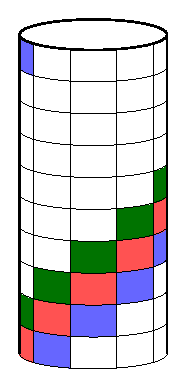
\includegraphics[width=.28\linewidth]{lb1-fig-19.pdf}
\FigureTag{LB1.19}{fig:lb1-19}
\end{figure}
Similarly, we finish colouring it; three colours are enough to visualize what he meant by colouring the cylinder diagonally in ten colours!
We have $41=4\times10+1$ pigeons (the rooks) in ten pigeonholes (the one-colour diagonals).
By P.H.P., there is at least one hole that contains at least $4+1=5$ pigeons.
But five rooks located on the same one-colour diagonal do not attack each other!
$(\text{Q.E.D.})^{\infty}$!
% Source page 38 - right
\setcounter{theorem}{78}\begin{lemma}[Angle sum of a triangle]\label{lemma:lb1-81}
The sum of all three angles in a triangle is $180^\circ$.
That is, if $ABC$ is a triangle, then $\angle A+\angle B+\angle C=180^\circ$.
\end{lemma}
The reason for writing this lemma is to present the following problem, which is truly marvellous.
\paragraph{Application.}
For George's 100th birthday party, he invited 202 guests.
They presented him with a rectangular birthday cake with, of course, 100 candles on it.
No three candles, two candles and a corner, or two corners and a candle were collinear.
George cuts the cake into triangular pieces by straight cuts connecting candles with each other and/or with corners of the cake, without any cut crossing previously made cuts, and every candle is used in a cut.
Prove that he ends up with exactly 202 pieces of cake.

Whew! That went too long, but let us make the solution a little short.
Let there be $n$ triangular pieces. Let us calculate the sum of all angles formed on that cake in two different ways.
The sum of the angles in a triangle is $180^\circ$, and there are $n$ triangles, so the angle sum is $180n$.
On the other hand, we get $360^\circ$ around every candle, plus four $90^\circ$ corners of the cake, making a total of $360\times100+90\times4$.
Thus $180n=360\times100+90\times4=180\times202$, so $n=202$.
Q.E.D.! Just like a piece of cake.


\subsection{Shovan's enigmatic perspective}
\paragraph{Balkan Mathematical Olympiad (2014).}
A regular hexagon of side $n$ is divided into unit equilateral triangles by lines parallel to its sides.
Count the regular hexagons in the resulting configuration.
Try the problem first. The more unsuccessful you are, the better you appreciate the solution!
We are thankful to the author, myself, for the following legendary solution.
% Source page 6 - right
\begin{figure}[H]\centering
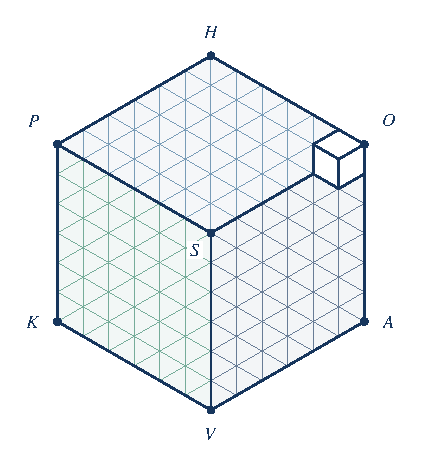
\includegraphics[width=.77\linewidth]{lb2-fig-04.pdf}
\FigureTag{LB2.4}{fig:lb2-04}
\end{figure}
``Extend the dimension.'' The source calls the drawing a ``$6^6$ cubical hexagon.''
Look carefully at $S$: $SPHOVAK$ is a cube.
Now look at the uncoloured unit hexagon near $O$; it also seems to be a small cube!
The unit hexagons are unit cubes in the first layer of the three faces facing us.
Similarly, the $k\times k$ hexagons correspond to unit cubes in the $k$th layer of those faces. Why?
Therefore the number of hexagons equals the number of unit cubes in an $n\times n\times n$ cube, namely $n^3$.
\emph{Quite a genius demonstration.}


\paragraph{What an amazing argument! WAAA!}
For a natural number $n$, prove
$\lfloor n/1\rfloor+\lfloor n/2\rfloor+\cdots+\lfloor n/n\rfloor+\lfloor\sqrt n\rfloor$ is even.
(INMO, 2014.)
% Source page 9 - right
In $P=\{1,2,\ldots,n\}$, the number of multiples of $q$ is $\lfloor n/q\rfloor$.
Counting multiples of $k$ not exceeding $n$ is equivalent to counting divisors of the numbers $1,\ldots,n$:
``Multiples are obtained by multiplying by a constant, and divisors by dividing by a constant.'' WAAA!
Thus $\sum_{k=1}^n\lfloor n/k\rfloor+\lfloor\sqrt n\rfloor
=\sum_{k=1}^n d(k)+\lfloor\sqrt n\rfloor$.
Now $d(k)\equiv1\pmod2$ exactly when $k$ is a perfect square, and $P$ contains $\lfloor\sqrt n\rfloor$ squares.
Therefore
$\sum_{k=1}^n\lfloor n/k\rfloor+\lfloor\sqrt n\rfloor
\equiv2\lfloor\sqrt n\rfloor\equiv0\pmod2$.
\emph{Quite intelligently done.}
% BLOG-CONTENT-END
\end{document}
